Nesta prática busca-se comparar os resultados do aprendizado ativo com o aprendizado supervisionado.

Realizamos dois experimentos com o classificador perceptron multicamadas agrupando as amostras em 5, o mesmo número de classes que devem ser inferidas.

No primeiro a seleção das amostras para ser aprezentada ao especialista foi feita escolhendo os pontos mais próximos do centróide. Mesmo com a utilização dos mesmos geradores de números aleatórios não foi possíve chegar ao valor de acurácia acima de 90\% obtidos nos experimentos supervisionado.

A partir da iteração 90 com 419 amostras rotuladas pelo especialista o desempenho tende a ficar constante como pode ser visto na Figura~\ref{fig:line_active_min}.

\begin{figure}[!htbp]
	\centering
	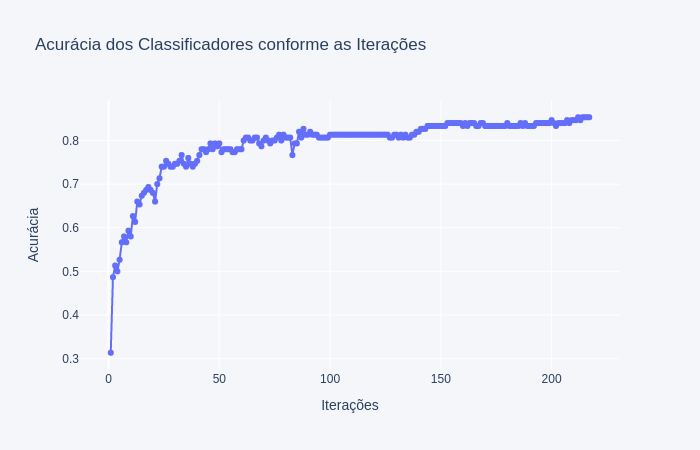
\includegraphics[width=1.0\linewidth,clip=true,trim=0cm 0cm 0cm 0cm, keepaspectratio=true]{line_active_min.png}
	\caption{Aprendizado Ativo: Número de iterações e acurácia. Seleção de pontos mais próximos do centróide.}
	\label{fig:line_active_min}
\end{figure}

Na segunda tentativa a seleção das amostras foi feita escolhendo os pontos mais distantes dos centróides. O resultado foi bem semelhante ao experimento anterior. A partira da iteração 90com 419 amostras rotuladas pelo especialista o desempenho tende a ficar constante como pode ser visto na Figura~\ref{fig:line_active_max}.

\begin{figure}[!htbp]
	\centering
	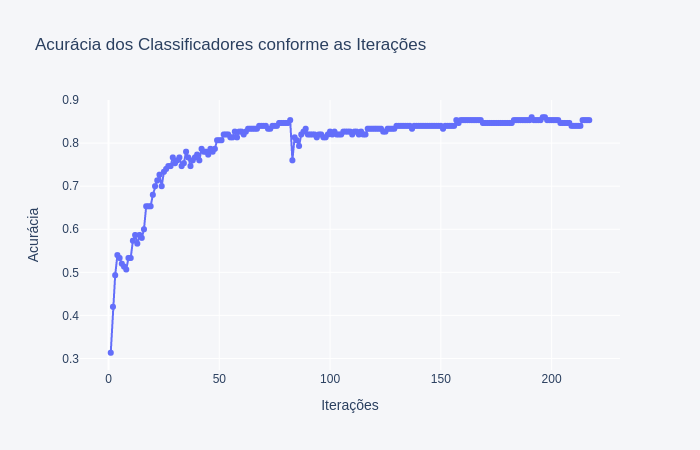
\includegraphics[width=1.0\linewidth,clip=true,trim=0cm 0cm 0cm 0cm, keepaspectratio=true]{line_active_max.png}
	\caption{Aprendizado Ativo: Número de iterações e acurácia. Seleção de pontos mais distantes do centróide.}
	\label{fig:line_active_max}
\end{figure}